\chapter{Grundlagen}\label{chap:Grundlagen}

\section{Mittelwert}\label{sec:Grundlagen:Mittelwert}
Der Mittelwert $\bar x$, auch genannt das Mittel oder auch der Durchschnitt, entspricht nach \autoref{eq:Mittelwert} der Summe der einzelnen Werte $x_1$, $x_2$, $x_3$ ... $x_n$ geteilt durch ihre Anzahl $n$.
\begin{equation}\label{eq:Mittelwert}
    \bar x = \frac{1}{n}\sum_{i=1}^n x_i
\end{equation}

\section{Susceptible-Infectious-Removed-Modell}\label{sec:Grundlagen:SIR}
Einen Weg zur Beschreibung einer Pandemie bietet das \glqq{}Susceptible-Infectious-Removed-Modell\grqq{} (SIR-Modell) \autocite{SIR}. Dieses Modell teilt die Mitglieder einer Menschengruppe in eine der drei folgenden Kategorien ein und ermöglicht es, die zeitliche Entwicklung einer Pandemie übersichtlich darzustellen:
\begin{itemize}
    \item \glqq{}Susceptible\grqq{}: Menschen, welche angesteckt werden können.
    \item \glqq{}Infectious\grqq{}: Infizierte Menschen, welche weitere Menschen anstecken können. Werden auch als \glqq{}die aktiven Fälle\grqq{} bezeichnet.
    \item \glqq{}Removed\grqq{}: Menschen, welche in die Kategorie \glqq{}Infectious\grqq{} fielen, nun keine weiteren Menschen mehr anstecken können und aus dem Infektionsgeschehen entfernt wurden,
    in diesem Fall Genesene und Verstorbene. 
\end{itemize}

Da nur die Zahlen der Kategorie \glqq{}Infectious\grqq{} direkt bereitgestellt werden, müssen die Zahlen der Kategorien \glqq{}Susceptible\grqq{} und \glqq{}Removed\grqq{} berechnet werden.

Die Zahl der Menschen in Kategorie \glqq{}Susceptible\grqq{} $S_t$ entspricht für das gewählte Gebiet $\Omega$ am Tag $t$ der Anzahl der Einwohner $p_{\Omega}$ abzüglich der akkumulierten Zahl der Fälle des Tages $F_t$ , wie in \autoref{eq:Susceptibles} angegeben. Diese Berechnung wird für jeden Tag $t$ durchgeführt, für den eine akkumulierte Zahl der Fälle $F_t$ angegeben ist.
    \begin{equation}\label{eq:Susceptibles}
        S_t=p_{\Omega}-F_t
    \end{equation}
Die Zahl der Menschen in Kategorie \glqq{}Removed\grqq{} $R_t$ für das gewählte Gebiet $\Omega$ am Tag $t$ ergibt sich aus der Summe der akkumulierten Anzahl der Genesenen $G_t$ und der akkumulierten Anzahl der Verstorbenen $V_t$. Sie wird ebenfalls nach \autoref{eq:Removed} für jeden Tag berechnet, für den die beiden Ausgangswerte vorliegen.
\begin{equation}\label{eq:Removed}
    R_t=G_t+V_t
\end{equation}

Die Zahlen der Kategorie \glqq{}Infectious\grqq{} liegen wie bereits erwähnt als aktive Fälle vor.

In dem hier verwendeten SIR-Modell wird weder die Geburten- noch die Sterberate beachtet, die angenomme Bevölkerung bleibt durchgehend konstant.

Zudem wird angenommen, dass jedes Individuum nur einmal infiziert werden kann und die Infektion die einzige Möglichkeit darstellt, von der Kategorie \glqq{}Susceptible\grqq{} in die Kategorie \glqq{}Removed\grqq{} zu wechseln.
Somit fällt die Zahl der Menschen in der Kategorie \glqq{}Susceptible\grqq{} monoton und die Zahl der Menschen in der Kategorie \glqq{}Removed\grqq{} steigt monoton an.\autocite{SIR}

\section{Bevölkerungsdichte}
Um für ein Gebiet $\Omega$ die Bevölkerungsdichte $\rho_{\Omega}$ zu berechnen, wird die Anzahl der Einwohner im Gebiet $p_{\Omega}$ durch die Fläche des Gebiets $A_{\Omega}$ geteilt:
\begin{equation}\label{eq:Bevölkerungsdichte}
    \rho_{\Omega} = \frac{p_{\Omega}}{A_{\Omega}}
\end{equation}
\section{7-Tage-Inzidenz}\label{sec:Grundlagen:7-Tages Inzidenz}
Die 7-Tage-Inzidenz ist die Zahl der neu gemeldeten Fälle in den letzten 7 Tagen pro 100~000 Menschen \autocite{7-TageInzidenz}.

Um die 7-Tage-Inzidenz $i_t$ für den Tag $t$ zu berechnen, wird von der akkumulierten Zahl der Fälle  am gewählten Tag $f_t$ die akkumulierte Zahl der Fälle sieben Tage zuvor $f_{t-7}$ abgezogen. Dies ergibt die neu hinzugekommenen Fälle innerhalb von sieben Tagen.

Schlussendlich wird diese Zahl durch die Anzahl der Bewohner des Gebiets $p_{Gebiet}$ geteilt und mit 100~000 multipliziert. Dies ergibt \autoref{eq:7-Tages_Inzidenz}.
\begin{equation}\label{eq:7-Tages_Inzidenz}
    i_t= \frac{f_t-f_{t-7}}{p_{\Omega}}\cdot 100~000
\end{equation}

Die 7-Tage-Inzidenz auf Basis der neu gemeldeten Fällen pro Tag bietet sich im Vergleich zu den aktiven Fällen oder der Todeszahl aus mehreren Gründen als Kennzahl für die Verbreitung eines Virus in einem Gebiet an:

Die neu gemeldeten Fallzahlen als Ausgangspunkt zu verwenden bietet sich im Gegensatz zu den aktiven Fällen an, da Beginn und Ende der Infektion bei den aktiven Fällen sehr schwer bestimmbar sind. Die Todeszahlen sind zwar eine gut bestimmbare Größe, jedoch würde hierbei ein größerer zeitlicher Verzug zur Infektion entstehen und generell kleinere Zahlen verwendet werden, welche auf Landkreisebene sehr viel anfälliger für Ausreißer wären.

In \autoref{fig:neue_Fälle_pro_Wochentag_Deutschland} werden die neu gemeldeten Fälle in Deutschland an unterschiedlichen Wochentagen dargestellt. Hierfür werden die einzelnen Wochen betrachtet und jeweils die Anzahl der am Montag gemeldeten Fälle von allen sieben Fallzahlen der Woche abgezogen. Dadurch ergeben sich die in \autoref{fig:neue_Fälle_pro_Wochentag_Deutschland} dargestellten gemeldeten Fälle am jeweiligen Wochentag relativ zu den gemeldeten Fällen an den Montagen.

Klar zu erkennen werden an Wochenenden im Schnitt deutlich weniger neue Fälle registriert als an den anderen Wochentagen.
Daher werden immer sieben Tage in der 7-Tage-Inzidenz zusammengefasst.
\begin{figure}[H]
    \centering
    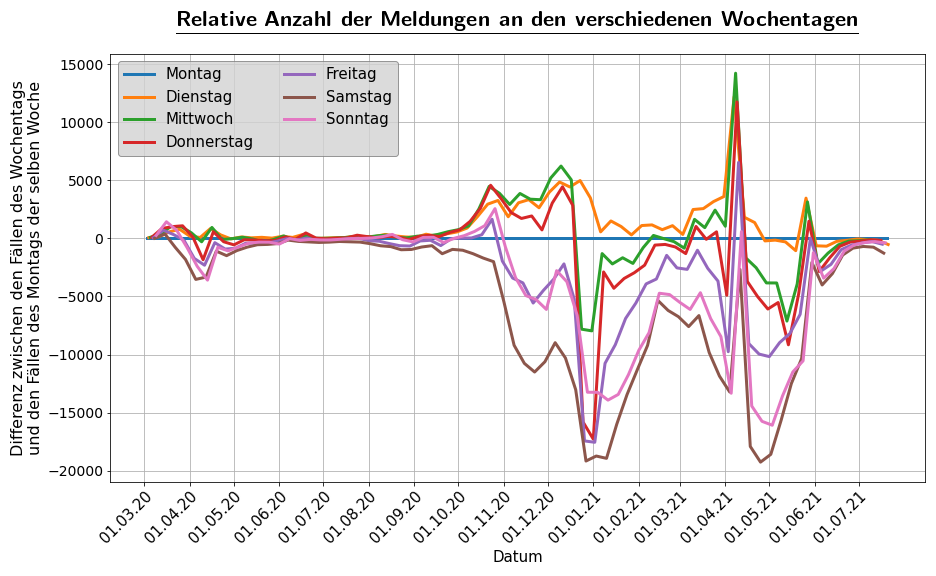
\includegraphics[width=\textwidth]{figures/Grundlagen/neue_Fälle_pro_Wochentag_Deutschland.png}
    \caption{In Deutschland neu gemeldete COVID-19-Fälle am jeweiligen Wochentag im Vergleich zu den am Montag der selben Woche gemeldeten Fälle.}
    \label{fig:neue_Fälle_pro_Wochentag_Deutschland}
\end{figure}
Da die Bevölkerung der deutschen Landkreise und Regierungsbezirke nicht identisch sind, wird jeweils durch die Bevölkerungszahl geteilt, um die einzelnen Gebiete miteinander vergleichen zu können.

\newpage
Aufgrund der ansonsten sehr kleinen Zahlen, bietet es sich zudem an, das Ergebnis mit 100~000 zu multiplizieren.

Dies sind die drei Begründungen für die drei Schritte in der Berechnung der 7-Tage-Inzidenz nach \autoref{eq:7-Tages_Inzidenz}.

\section{Lexikographische Ordnung}\label{sec:Grundlagen:lexikographisch}
Um mehrere Zahlen in eine lexikographische Ordnung zu bringen, werden die Zahlen zuerst nach der ersten Ziffer sortiert. Anschließend werden die Zahlen mit der selben ersten Ziffer nach der zweiten Ziffer sortiert. Anschließend werden die Zahlen mit der selben zweiten Ziffer nach der dritten Ziffer sortiert und so weiter.

Dadurch ergibt sich eine Ordnung, bei welcher beispielsweise 1000 vor 200 kommt. Als Beispiel bietet sich die Liste der Landkreise in \autoref{tab:counties_by_admunitid}, die Landkreise sind hierbei lexikographisch nach dem Gemeindeschlüssel sortiert.
\section{Korrelationsanalyse mithilfe einer Faltung}\label{sec:BeschreibungKorrelationsanalyse}
\subsection{Berechnung der Korrelationswerte}\label{sec:Grundlagen:BerechnungderKorrelationwertes}
Um festzustellen, ob die 7-Tage-Inzidenzen einiger Landkreise im Vergleich zu anderen Landkreisen eher voraus- oder nacheilen, werden die Korrelationswerte im Rahmen der nachfolgend vorgestellten Korrelationsanalyse berechnet \autocite{Korrelation}.

Bei diskreten Werten, aufgeteilt in zwei Zeitreihen $X:|X|=n$ und $Y:|Y|=n$ mit den Werten $x_t$ und $y_t$, wie in diesem Fall, basiert die Korrelationsanalyse auf einer diskreten Faltung $X\ast Y$:
Für eine zeitliche Verschiebung $\tau$ wird mit jedem Wert $x_t$ zum jeweiligen Zeitpunkt $t$ aus der ersten Zeitreihe mit dem zugehörigen Wert $y_{t+\tau}$ aus der zweiten Zeitreihe ein Produkt gebildet. Der zugehörige Wert aus der zweiten Zeitreihe entspricht hierbei dem Zeitpunkt $t$ des Wertes der ersten Zeitreihe plus der gewählten Verschiebung $\tau$. Sollte dieser zweite Wert nicht existieren, wird kein Produkt gebildet.

Für jede zeitliche Verschiebung $\tau$, für die mindestens ein Produkt gebildet wird, werden wie in \autoref{eq:Korrelation} alle möglichen Produkte aufsummiert.
\begin{equation}\label{eq:Korrelation}
    X\ast Y = \sum_{t=1}^n x_t\cdot y_{t+\tau}
\end{equation}


Bildlich gesprochen wird die zweite Zeitreihe an der ersten Zeitreihe vorbeigeschoben, beginnend an dem Punkt, an dem ausschließlich das erste Element der ersten Zeitreihe mit dem letzten Element der zweiten Zeitreihe multipliziert wird. Dies ist beispielhaft mit den Folgen $[1,2,3,2]$ und $[5,7,5,1]$ in \autoref{fig:Korrelation Beispiel} dargestellt.

\begin{figure}[H]
    \centering
    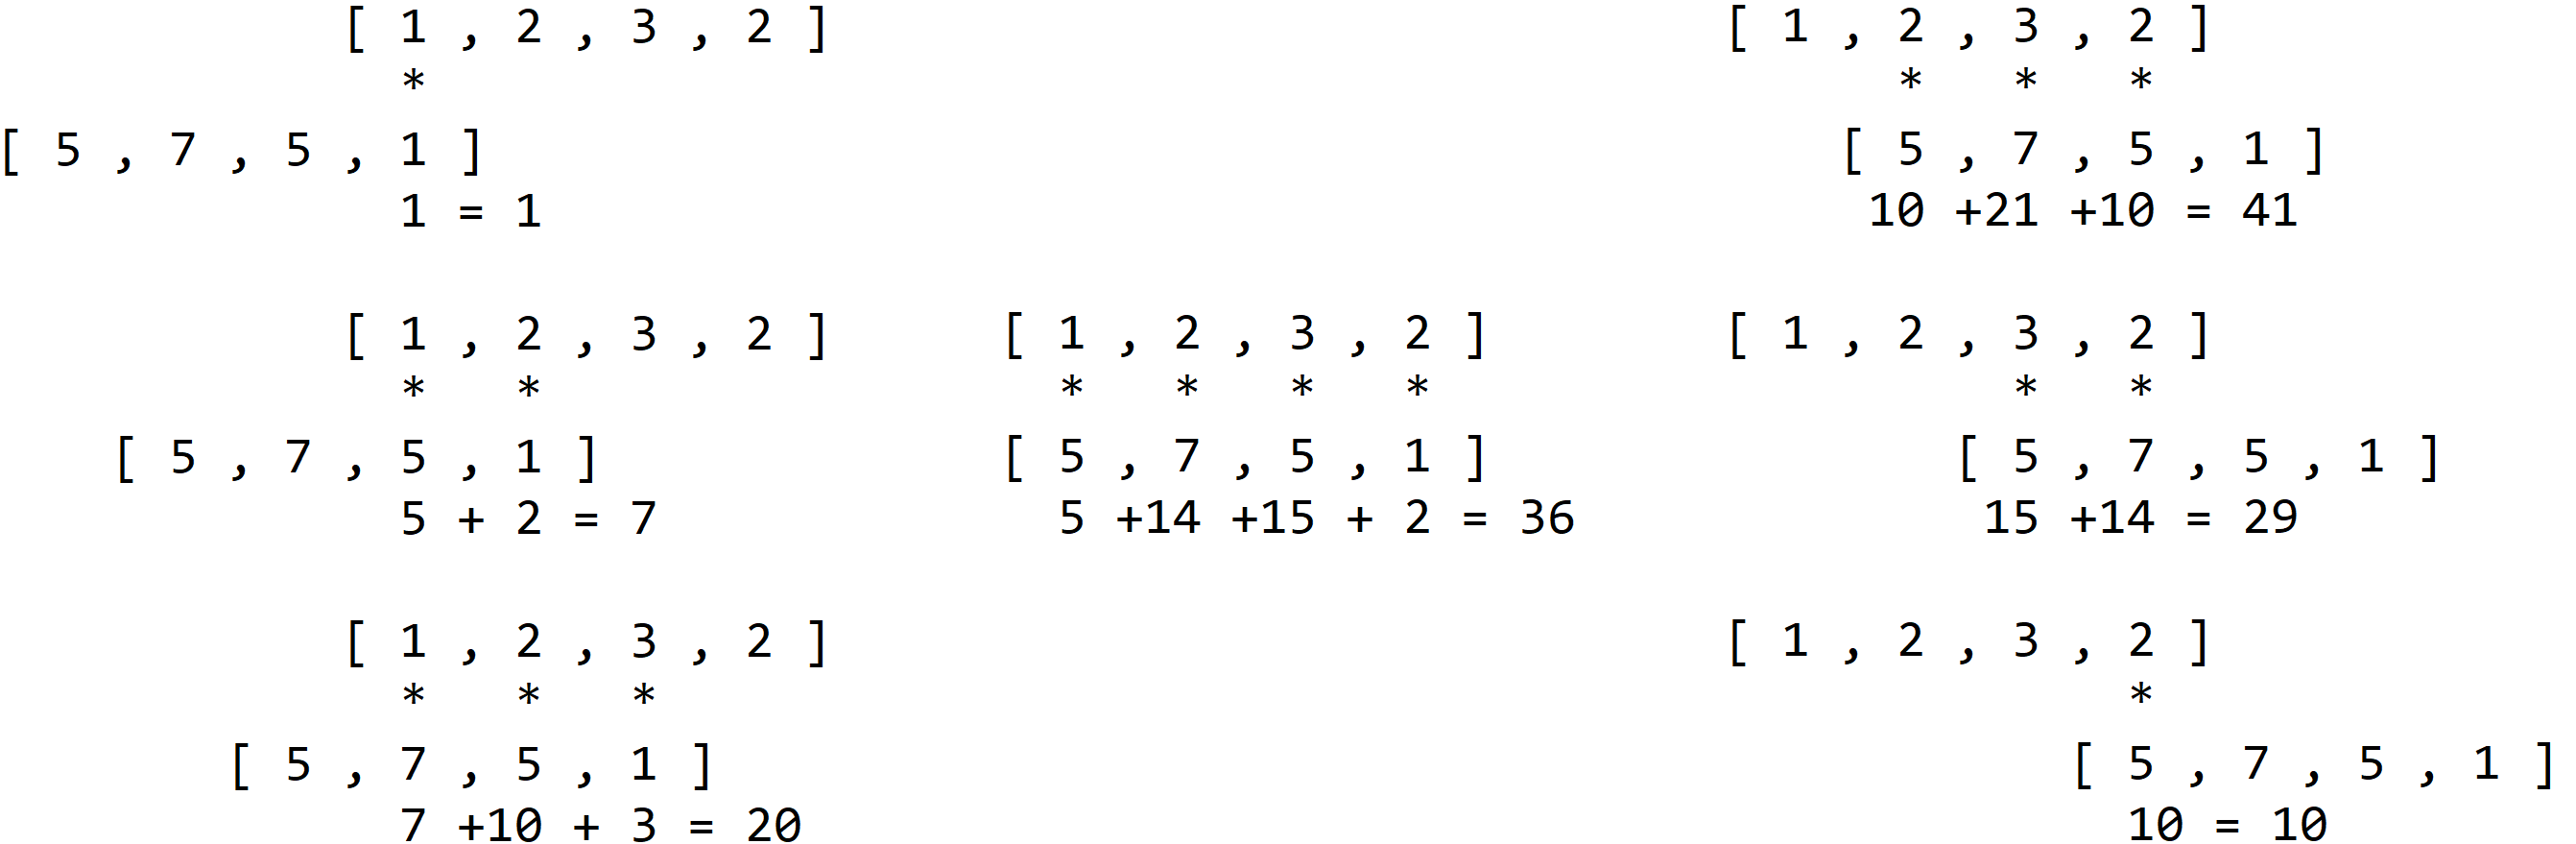
\includegraphics[width=\textwidth]{figures/Grundlagen/Korrelation.png}
    \caption{Beispielhafte Darstellung einer Faltung anhand der Folgen $[1,2,3,2]$ und $[5,7,5,1]$. Auf der linken Seite sind von oben nach unten hinter dem Gleichheitszeichen die Korrelationswerte für die negativen Verschiebungen $\tau=-3$, $\tau=-2$ und $\tau=-1$ eingetragen. Entsprechend sind der Korrelationswert für die Verschiebung $\tau=0$ in der Mitte und die Korrelationswerte für die positiven Verschiebungen $\tau=1$, $\tau=2$ und $\tau=3$ auf der rechten Seite zu finden.}
    \label{fig:Korrelation Beispiel}
\end{figure}

Da bei einer Korrelationsanalyse nach \autoref{eq:Korrelation} Summen aus mehr Produkten übergewichtet werden und Zeitreihen mit größeren Werten größere Korrelationswerte erzeugen, müssen die Korrelationswerte noch skaliert werden.

Um zum einen die unterschiedliche Anzahl der Produkte auszugleichen, werden die Summen durch die Anzahl ihrer Summanden geteilt, wie in \autoref{eq:skalierte_Korrelation_geteilt_durch_Produkte} gezeigt. Ohne diese Gewichtung würden zwei Zeitreihen mit konstanten Werten größer null bei einer Verschiebung $\tau=0$ die größte Korrelation aufweisen und die Korrelation bei betragsmäßig größeren Verschiebungen abnehmen, was nicht gewünscht ist.

Da jede Zeitreihe die gleiche Länge $n$ hat, erhält man die Anzahl der Summanden $m$, indem man
den Betrag der Verschiebung $\vert\tau\vert$
von der Länge der Zeitreihe $n$ abzieht, somit ergibt sich die Rohform einer Korrelationsanalyse $\hat{c}(\tau)$:

\begin{equation}\label{eq:skalierte_Korrelation_geteilt_durch_Produkte}
    \hat{c}(\tau) =\frac{1}{m} \sum_{t=1}^n x_t\cdot y_{i+\tau}=\frac{1}{n-\vert\tau\vert} \sum_{t=1}^n x_t\cdot y_{i+\tau}
\end{equation}

Um zum anderen die tendenziell größeren Werte mancher Zeitreihen auszugleichen, werden die Werte aller Zeitreihen mithilfe des sogenannten \glqq{}Autokorrelationswerts für die Verschiebung $\tau=0$ gewichtet: Er beschreibt den Wert der Korrelation einer Zeitreihe mit sich selbst bei keiner zeitlichen Verschiebung. Wie in \autoref{eq:skalierte_Korrelation} zu sehen, werden die Werte einer Zeitreihe gewichtet, indem sie durch die Wurzel des Autokorrelationswerts für die Verschiebung $\tau=0$ dieser Zeitreihe geteilt werden.

\begin{equation}\label{eq:skalierte_Korrelation}
    c(\tau) =
    \frac{1}{n-\vert\tau\vert}
    \sum_{t=1}^n
    \frac{x_t}{\sqrt{\frac{1}{n}\sum_{t=1}^n x_t^2}}
    \cdot
    \frac{y_{t+\tau}}{\sqrt{\frac{1}{n}\sum_{t=1}^n y_t^2}}
    =
    \frac{n}{n-\vert\tau\vert}
    \frac{\sum_{t=1}^n x_t \cdot y_{t+\tau}}
    {\sqrt{\sum_{t=1}^n x_t^2}
    \sqrt{\sum_{t=1}^n y_t^2}}
\end{equation}


Zudem wird von jedem Wert $x_t$ der Zeitreihe der Mittelwert $\overline x = \frac{1}{n}\sum_{t=1}^n x_t$ abgezogen. Dadurch lassen sich Antikorrelationen feststellen: Wenn beispielsweise die Anzahl der COVID-19-Infektionen eines Landkreises zu einem Zeitpunkt überdurchschnittlich wächst, also die 7-Tage-Inzidenz minus dem Mittelwert der 7-Tage-Inzidenzen positiv ist, und das andere Edukt aus der anderen Zeitreihe negativ ist, also in dem anderen Landkreis die Anzahl der COVID-19-Infektionen unterdurchschnittlich wächst, ergibt sich ein negatives Produkt, da sich die Situation in dem einen Landkreis  schneller als üblich verschlechtert, während sich die Situation im anderen Landkreis verbessert oder langsamer als üblich verschlechtert.

Ergibt die Summe aus all den Produkten einer Korrelation eine negative Zahl, scheint die 7-Tage-Inzidenz des einen Landkreises zu fallen oder langsam zu steigen, während die 7-Tage-Inzidenz des anderen Landkreises steigt oder langsam fällt, dies wird hier Antikorrelation genannt.

Mit allen Ergänzungen berechnet sich die Korrelation $c(\tau)$ zwischen der Zeitreihe $X:|X|=n$ mit den Werten $x_t\in X$ und der Zeitreihe $Y:|Y|=n$ mit den Werten $y_t \in Y$ und einer Verschiebung $\tau$ relativ zu $X$ mithilfe der Mittelwerte der Zeitreihen $\overline x,\ \overline y$ wie in \autoref{eq:komplette_skalierte_Korrelation} beschrieben.
\begin{equation}\label{eq:komplette_skalierte_Korrelation}
    c(\tau) =\frac{n}{n-\vert\tau\vert}
    \frac{\sum_{t=1}^n (x_t-\overline x)\cdot (y_{t+\tau}-\overline y)}{\sqrt{\sum_{t=1}^n (x_t-\overline x)^2}\sqrt{\sum_{t=1}^n (y_t-\overline y)^2}}
\end{equation}

\subsection{Korrelation zwischen zwei Gebieten am Beispiel von Flensburg und Kiel}
Um die verwendete Terminologie und die hergeleiteten Gleichungen anhand eines Beispiels näher zu bringen, werden in diesem Abschnitt die einzelnen Schritte einer Korrelationsanalyse ausgeführt. Als Beispiel dient hierfür die Korrelation zwischen dem Verlauf der 7-Tage-Inzidenzen der Stadtkreise Flensburg und Kiel. Die Daten stammen aus dem \glqq{}COVID-19 Datenhub\grqq{}
(\href{npgeo-corona-npgeo-de.hub.arcgis.com}{npgeo-corona-npgeo-de.hub.arcgis.com}), weitere Informationen zur Datenquelle und der Datenbeschaffung folgen in \autoref{chap:Vorgehensweise}.

Beide Verläufe bestehen aus 508 7-Tage-Inzidenzen, welche jeweils einem Tag zugeordnet sind. Die 7-Tage-Inzidenzen sind in \autoref{fig:Inzidenz_Flensburg} und \autoref{fig:Inzidenz_Kiel} abgebildet, jeweils einmal im Original und einmal um den Mittelwert der 7-Tage-Inzidenz in x-Richtung nach unten verschoben.

\begin{figure}[H]
    \centering
    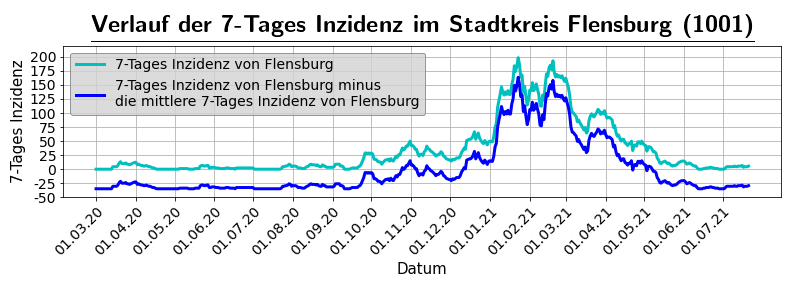
\includegraphics[width=\textwidth]{figures/Grundlagen/Inzidenz_Flensburg.png}
    \caption{Der Verlauf der 7-Tage-Inzidenz des Stadtkreises Flensburg (Gemeindeschlüssel 1001).
    In Türkis ist der originale Verlauf der 7-Tage-Inzidenz dargestellt. Der Verlauf der 7-Tage-Inzidenzen, von denen der Mittelwert der 7-Tage-Inzidenzen von Flensburg abgezogen wurde, ist Blau dargestellt.}
    \label{fig:Inzidenz_Flensburg}
\end{figure}
\begin{figure}[H]
    \centering
    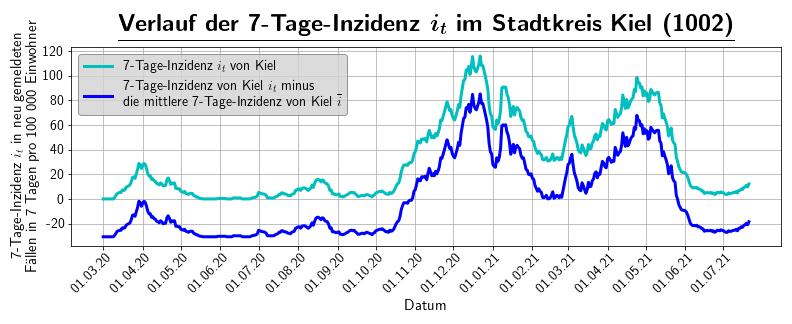
\includegraphics[width=\textwidth]{figures/Grundlagen/Inzidenz_Kiel.png}
    \caption{Der Verlauf der 7-Tage-Inzidenz des Stadtkreises Kiel (Gemeindeschlüssel 1002).
    In Türkis sind ist der originale Verlauf der 7-Tage-Inzidenz dargestellt. Der Verlauf der 7-Tage-Inzidenzen, von denen der Mittelwert der 7-Tage-Inzidenzen von Kiel abgezogen wurde, ist Blau dargestellt.}
    \label{fig:Inzidenz_Kiel}
\end{figure}
In \autoref{fig:correlation_Flensburg_Kiel} ist die diskrete Faltung abgebildet, wie sie der Korrelationsanalyse zugrunde liegt und in \autoref{eq:Korrelation} definiert ist.
\newpage
Die Faltung der beiden in \autoref{fig:Inzidenz_Flensburg} und \autoref{fig:Inzidenz_Kiel} gezeigten Zeitreihen der Länge 508 erzeugt 1015 Werte, da das Spektrum der Verschiebungen $\tau$ bei $\tau=-507$ beginnt und die ganzen Zahlen bis einschließlich $\tau=507$ enthält.
Für jeden der 412 Landkreise ergeben sich daher aus der Korrelationsanalyse mit sich selbst und jedem anderen Landkreis 418~180 Werte, ebenso ergeben sich für jeden der 38 Regierungsbezirke 38~570. Dies ergibt in Summe 
%38.570\cdot 38 + 418.180\cdot412 = 1.465.660+172.290.160=
173~755~820 Werte.
\begin{figure}[H]
    \centering
    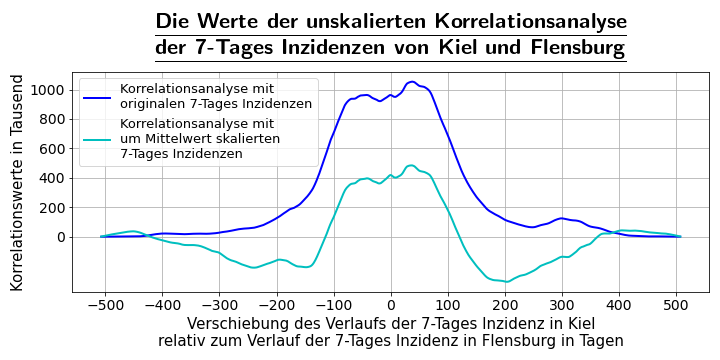
\includegraphics[width=\textwidth]{figures/Grundlagen/correlation_Flensburg_Kiel.png}
    \caption{Ergebnis der diskreten Faltung der 7-Tage-Inzidenzen der Stadtkreise Kiel und Flensburg.
    In Türkis ist das Ergebnis der Faltung mit den originalen 7-Tage-Inzidenzen dargestellt. Das Ergebnis der Faltung mit den 7-Tage-Inzidenzen, von denen der Mittelwert der 7-Tage-Inzidenzen des jeweiligen Landkreises abgezogen wurde, ist Blau dargestellt.}
    \label{fig:correlation_Flensburg_Kiel}
\end{figure}
\autoref{fig:correlation_Flensburg_Kiel_scaled_autocorrelation} ergibt sich, wenn die Summen jeweils durch die Anzahl ihrer Summanden (den Produkten) geteilt werden, wie in \autoref{eq:skalierte_Korrelation_geteilt_durch_Produkte} beschrieben. Klar zu erkennen sind die verstärkten Ausschläge am linken und rechten Rand. Sie entstehen dadurch, dass bei betragsmäßig größeren Verschiebungen der Divisor $n-\vert\tau\vert$ kleiner wird. Dadurch werden die einzelnen Produkte stärker gewichtet und Abweichungen einzelner Produkte sorgen für größere Ausschläge.
\begin{figure}[H]
    \centering
    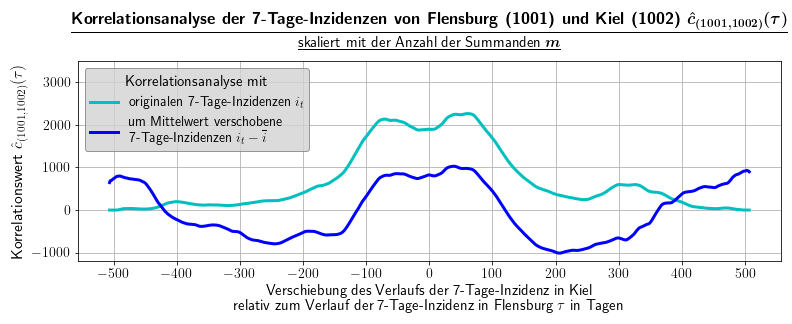
\includegraphics[width=\textwidth]{figures/Grundlagen/correlation_Flensburg_Kiel_scaled_autocorrelation.png}
    \caption{Korrelationsanalyse der 7-Tage-Inzidenzen der Stadtkreise Kiel und Flensburg ohne Skalierung mithilfe der Autokorrelation.
    In Türkis ist das Ergebnis der Korrelationsanalyse mit den originalen 7-Tage-Inzidenzen dargestellt. Das Ergebnis der Korrelationsanalyse mit den 7-Tage-Inzidenzen, von denen der Mittelwert der 7-Tage-Inzidenzen des jeweiligen Landkreises abgezogen wurde, ist Blau dargestellt.}
    \label{fig:correlation_Flensburg_Kiel_scaled_autocorrelation}
\end{figure}
In \autoref{fig:correlation_Flensburg_Kiel_scaled_autocorrelation} sind die Ergebnisse der kompletten Korrelationsanalyse abgebildet, wie sie mithilfe von \autoref{eq:skalierte_Korrelation} erzeugt werden.
\begin{figure}[H]
    \centering
    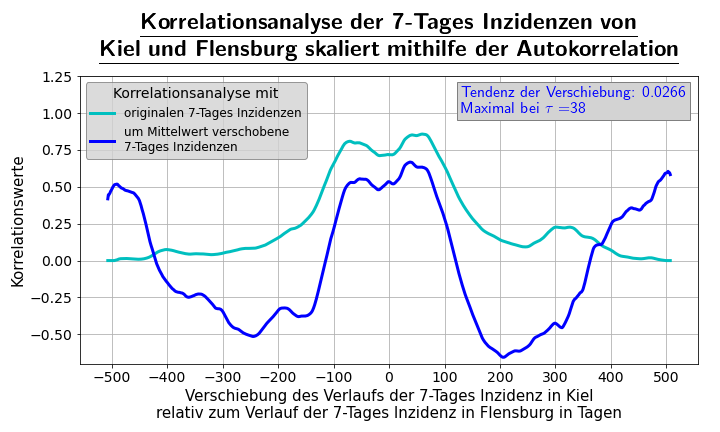
\includegraphics[width=\textwidth]{figures/Grundlagen/correlation_Flensburg_Kiel_scaled_complete.png}
    \caption{Vollständige Korrelationsanalyse der 7-Tage-Inzidenzen der Stadtkreise Kiel und Flensburg skaliert mithilfe der Autokorrelation.
    In Türkis ist das Ergebnis der Korrelationsanalyse mit den originalen 7-Tage-Inzidenzen dargestellt. Das Ergebnis der Korrelationsanalyse mit den 7-Tage-Inzidenzen, von denen der Mittelwert der 7-Tage-Inzidenzen des jeweiligen Landkreises abgezogen wurde, ist Blau dargestellt.}
    \label{fig:correlation_Flensburg_Kiel_scaled_complete}
\end{figure}

Jeder Korrelationswert gibt den Grad des linearen Zusammenhangs bei der jeweiligen Verschiebung an, wobei die zugeordneten Verschiebungen von links nach rechts bei jedem Schritt um eins zunehmen und der mittlere der Korrelationswerte der Verschiebung $\tau = 0$ zugeordnet ist. Die Verschiebung ist im Kontext dieser Arbeit stets in ganzen Tagen zwischen $-507$ und $507$ angegeben. 

\subsection{Komprimierung und Darstellung als Matrizen}\label{sec:Grundlagen:Korrelation:Komprimierung}
Das Ziel der nachfolgend beschriebenen Schritte ist, die Korrelationswerte eines Gebiets auf einen Wert zusammenzuführen. Dadurch kann man einfach und schnell auffallende Korrelationen zwischen zwei oder mehreren Gebieten finden und erhält einen besseren Überblick über die 173~755~820 ermittelten Korrelationswerte.
Hierfür werden zwei Methoden verwendet:
\begin{itemize}
    \item Die Verschiebung $\tau_0$ mit dem maximalen Korrelationswert $c(\tau_0)$: Die zeitliche Verschiebung, bei der die Korrelationsanalyse den größten Korrelationswert ergeben hat.
    \item Die Tendenz der Verschiebung $\hat{\tau}$: 
    Das Mittel der Differenz zwischen den Werten der betragsmäßig gleichen Verschiebungen.
    Das Resultat ermöglicht eine grobe Einschätzung, ob der maximale Wert nur ein Ausreißer ist oder nicht.
\end{itemize}

Die Berechnung der Tendenz der Verschiebung $\hat{\tau}$ ist etwas komplexer und wird daher ebenfalls am Beispiel der Korrelationsanalyse der Stadtkreise Kiel und Flensburg erklärt.
In \autoref{fig:Flensburg_Kiel_Verschiebung_Tendenz} ist die Berechnung graphisch dargestellt.
Die Tendenz der Verschiebung $\hat{\tau}$ berechnet sich aus der Liste der Korrelationswerte $C:\vert C\vert =m$, genauer gesagt aus ihrer Länge $m$ und ihren Werten $c_\tau$,$ -\lfloor m/2 \rfloor\geq \tau\leq \lfloor m/2 \rfloor$:
\begin{equation}\label{eq:Tendenz der Verschiebung}
    \hat{\tau} = \frac{1}{\lfloor m/2 \rfloor}
    \sum_{\tau=1}^{\lfloor m/2 \rfloor}c_{\tau}-c_{-\tau}
\end{equation}
\newpage
In \autoref{fig:Flensburg_Kiel_Verschiebung_Tendenz} entspricht der blaue Graph den Werten der Korrelationsanalyse wie sie auch in \autoref{fig:correlation_Flensburg_Kiel_scaled_complete} abgebildet sind. Um bildlich die Differenz zwischen den Werten der betragsmäßig gleichen Verschiebungen darzustellen, werden die Werte der negativen Verschiebungen an der Vertikalen bei $x=0$ gespiegelt und Lila eingefärbt.
Da die linke Seite gespiegelt wird, ist sie nicht weiter von Bedeutung.

In den Zwischenräumen der beiden Graphen und auf der Horizontalen bei $y=0$ sind die Differenzen der Werte der betragsmäßig gleichen Verschiebungen aufgezeichnet, deren Mittel der Tendenz der Verschiebung entspricht. Diese ist als dunkelblaue Horizontale bei $y=0.0266$ dargestellt.

\begin{figure}[H]
    \centering
    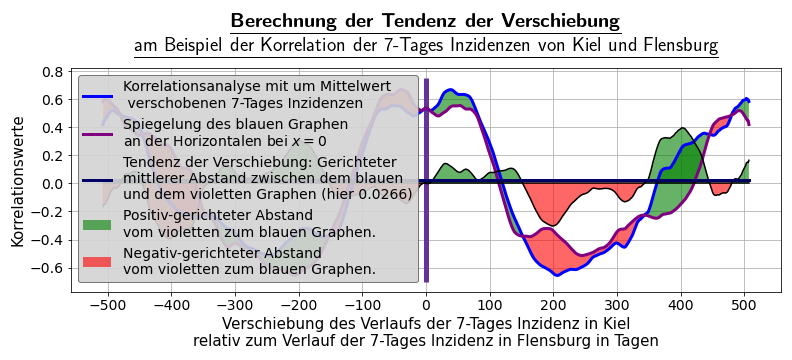
\includegraphics[width=\textwidth]{figures/Grundlagen/correlation_Flensburg_Kiel_Verschiebung_Tendenz.png}
    \caption{Graphische Darstellung der Berechnung der Tendenz der Verschiebung.}
    \label{fig:Flensburg_Kiel_Verschiebung_Tendenz}
\end{figure}

Somit lässt sich zum einen die Verschiebung mit dem maximalen Korrelationswert ermitteln und einfach interpretieren.
Da hierfür jedoch nur ein Wert herausgenommen wird, bietet es sich zum anderen an, die Tendenz der Verschiebung zu berechnen und mit der Verschiebung mit dem maximalen Korrelationswert zu vergleichen.



Um dies für alle Landkreise und Regierungsbezirke zu ermöglichen, werden die beiden Werte jeweils in einer Matrix dargestellt: Jeder Zeile und Spalte wird der Index für ein Gebiet zugeordnet. In die Zellen werden entweder die Verschiebungen mit dem maximalen Korrelationswert oder die Tendenzen der Verschiebung eingetragen. Ein spezifischer Wert in einer Zelle stammt aus der Korrelationsanalyse der Gebiete, die der Zeile und der Spalte zugeordnet sind.
Die Matrizen sind (mit umgekehrtem Vorzeichen) symmetrisch an der Diagonalen von links oben nach rechts unten. Die Diagonalen sind mit Nullen besetzt, da die Werte der positiven Verschiebung symmetrisch zu den Werten der negativen Verschiebung sind und die Korrelation mit sich selbst trivialerweise bei einer Verschiebung von $\tau=0$ am größten ist, da die Werte und Trends komplett identisch sind.

Um den Gebieten selbst Werte zuzuordnen und nicht nur in Kombination mit einem anderen Gebiet, wird sowohl bei den Maximalwerten wie auch den Tendenzen der Verschiebung der Mittelwert gebildet, indem die Zeilen der Matrizen aufsummiert werden und durch die Anzahl der Spalten geteilt werden.
\newpage
\section{Farbgebung}\label{sec:Grundlagen:Farbgebung}
Um schnell verständliche Abbildungen bereitstellen zu können, werden die Werte skaliert und die Farbgebung der Deutschlandkarten derart angepasst, dass das gesamte Farbspektrum abgedeckt wird. Das Farbspektrum reicht von blau über grün zu gelb zu rot, wie in \autoref{fig:color_schemes} demonstriert. Die niedrigsten Werte werden blau gefärbt und in der Regel die weiteren Farben linear zugeordnet, bis dem höchsten Wert schwarz zugeteilt wird.
Das bedeutet, dass einer Zahlenfolge mit 30 Zahlen mit selbem Abstand zueinander exakt die 30 in \autoref{fig:color_schemes} dargestellten Farben zugeordnet werden.
Da manche dieser Farbwerte im Kontrast zu einem weißen Hintergrund schwer zu erkennen sind, ist der Hintergrund der meisten Abbildungen grau.

\begin{figure}[H]
    \centering
    
\includegraphics[width=0.8\textwidth]{figures/Grundlagen/color_schemes.png}
    \caption{Das Farbspektrum, in welchem sich die Darstellungen bewegen. Von links nach rechts steigen die eingegebenen Werte äquidistant. Der angegebene Wert wird jeweils anhand des ersten und des letzten Wertes linear in diesem Spektrum verortet.}
    \label{fig:color_schemes}
\end{figure}

Die Matrizen werden durch die verwendete Python-Programmbibliothek \glqq{}Matplotlib\grqq{} automatisch eingefärbt.